
% Copyright 2022 by Robert Hildebrand
%This work is licensed under a
%Creative Commons Attribution-ShareAlike 4.0 International License (CC BY-SA 4.0)
%See http://creativecommons.org/licenses/by-sa/4.0/

\chapter{Duality}
\label{ch:duality}

\begin{outcome}
You will learn
\begin{itemize}
\item How to derive a bound on the optimal objective value
\item How to reformulate the problem into a \emph{dual} with a different interpretation
\item Correspondence between the primal (original) and dual problems
\end{itemize}
\end{outcome}

\begin{tryit}
\vizlink{dual-construction}{Primal-to-Dual Construction}: build the dual one multiplier at a time, exactly as in this chapter.

\vizlink{duality-sensitivity}{Duality and Sensitivity Explorer}: the primal, the dual, and the shadow prices, live.

\vizlink{dual-simplex}{Dual Simplex Method}: a further topic to explore after this chapter.
\end{tryit}



\begin{quote}
\itshape A rival baker knocks on your door with an offer: ``Don't bake tomorrow. Sell me your whole pantry (every unit of flour and sugar) and take the day off.'' You would only accept if the payment beats every plan you could bake yourself, so the rival must price each ingredient carefully: the ingredients that go into one cake must fetch at least a cake's profit, and likewise for cookies; otherwise you would simply say no and bake. The rival, of course, wants the cheapest offer that convinces you. That cheapest convincing offer turns out to equal your best baking profit \emph{exactly}. Finding the rival's prices is a linear program too: the \emph{dual} of yours.
\end{quote}

\section{Duality Theory}
\label{sec:duality-theory}

\subsection*{Motivating Example}

Imagine you run a small bakery that makes two products: cakes ($x_1$) and cookies ($x_2$). Your goal is to maximize your daily profit. Cakes yield a profit of \$3 each, and cookies yield \$2 each. You are limited by the ingredients you have on hand: you have at most 4 units of flour and 5 units of sugar available each day. Each cake requires 1 unit of flour and 2 units of sugar, while each cookie requires 1 unit of flour and 1 unit of sugar. We can write this scenario as a linear program:

\[
\begin{aligned}
\max \; & 3x_1 + 2x_2 && \text{(maximize total profit)}\\
\text{subject to } & x_1 + x_2 \leq 4 && \text{(flour constraint)}\\
& 2x_1 + x_2 \leq 5 && \text{(sugar constraint)}\\
& x_1, x_2 \geq 0.
\end{aligned}
\]

Here, $x_1$ is the number of cakes you bake, and $x_2$ is the number of cookies. The constraints limit how many of each product you can produce given your resources.

Now, suppose a friend is not sure that you are telling the truth about the maximum profit you can make. They ask, ``Can you prove an upper bound on how much money you could possibly earn with these ingredient constraints, without actually solving the problem?''

\subsection*{Intuition Behind Duality}

Consider the constraints in the problem. Each one puts a cap on how large the combination of $x_1$ and $x_2$ can be. If we think of them separately:

\begin{itemize}
\item The flour constraint: $x_1 + x_2 \leq 4$.
\item The sugar constraint: $2x_1 + x_2 \leq 5$.
\end{itemize}
Now, what if we take some nonnegative multipliers $y_1$ and $y_2$ and combine these inequalities into one single inequality? For instance, multiply the flour constraint by $y_1 \geq 0$ and the sugar constraint by $y_2 \geq 0$ and add them up:

\[
y_1(x_1 + x_2) + y_2(2x_1 + x_2) \leq y_1(4) + y_2(5).
\]

Grouping the terms by $x_1$ and $x_2$ gives:

\[
(x_1(y_1 + 2y_2)) + (x_2(y_1 + y_2)) \leq 4y_1 + 5y_2.
\]

If we choose $y_1$ and $y_2$ cleverly, we can force the left-hand side to be an expression that is always \emph{at least} as large as our profit function $3x_1 + 2x_2$. Specifically, we want

\[
y_1 + 2y_2 \geq 3 \quad \text{and} \quad y_1 + y_2 \geq 2.
\]

Why? Because if the coefficients on $x_1$ and $x_2$ in our combined inequality dominate those in our profit function, then the upper bound on the combined inequality's right-hand side ($4y_1 + 5y_2$) will also serve as an upper bound on the profit $3x_1 + 2x_2$. This ensures:

\[
3x_1 + 2x_2 \leq (y_1+2y_2)x_1 + (y_1 + y_2)x_2 \leq 4y_1 + 5y_2.
\]

Thus, by choosing $y_1$ and $y_2$, we obtain a valid upper bound on the maximum profit. If we try to minimize $4y_1 + 5y_2$ over all $y_1, y_2 \geq 0$ that satisfy these inequalities, we find the best (smallest) upper bound on our original problem.

The whole argument is a pipeline: it starts from the constraints you already have and ends at a new optimization problem.  Figure~\ref{fig:duality-pipeline} summarizes it.  The key step is the last one: searching for the \emph{best} certificate is itself a linear program.

\begin{figure}[h!]
\centering
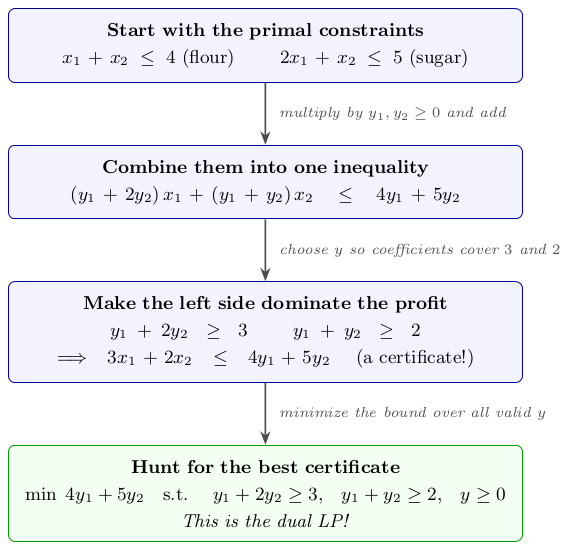
\includegraphics[width=3.84in]{figs/duality-tikz01.png}
\caption{From constraints to the dual: every feasible $y$ certifies an upper bound on profit, and the dual LP finds the best certificate.}
\label{fig:duality-pipeline}
\end{figure}

\begin{learningcheckpoint}[label={lc:duality-certificate}]
In the bakery problem, take multipliers $y_1 = 3$ and $y_2 = 0$.  Verify that this choice satisfies both dominance conditions, and compute the resulting upper bound on profit.  Then compare it with the bound from $y_1 = 1,\, y_2 = 1$.  Which certificate is better?  Can you find one better still?
\end{learningcheckpoint}

\subsection*{General Derivation of the Dual}

We started with the primal problem in a general form:

\[
\begin{aligned}
\max \; & \c^\top \x \\
\text{subject to } & A\x \leq \b \\
& \x \geq 0.
\end{aligned}
\]

Each constraint $a^i \cdot x \leq b_i$ (where $a^i$ is the $i$-th row of $A$) is valid for all feasible $x$. If we take a nonnegative combination of these constraints, say with multipliers $y_i \geq 0$, we get:

\[
\sum_{i=1}^m y_i (a^i \cdot \x) \leq \sum_{i=1}^m y_i b_i.
\]

This can be written as:

\[
(\sum_{i=1}^m y_i \a^i) \cdot \x \leq \sum_{i=1}^m y_i b_i.
\]

If we choose $\y$ such that $\sum_{i=1}^m y_i a^i \geq c$, then for all feasible $\x$ (since $\x \geq 0$):

\[
\c^\top \x \leq (\sum_{i=1}^m y_i a^i)\cdot \x \leq \sum_{i=1}^m y_i b_i.
\]

So, $\b^\top \y = \sum_{i=1}^m y_i b_i$ is an upper bound on the maximum primal objective value. By minimizing over all such $y$, we seek the tightest upper bound:

\[
\begin{aligned}
\min \; & \b^\top \y \\
\text{subject to } & A^\top \y \geq \c \\
& \y \geq 0.
\end{aligned}
\]

This is the \emph{dual} problem. In our bakery scenario, this dual formulation corresponds to adjusting the prices (the $y$ values can be thought of as ``shadow prices'') you would assign to each ingredient such that if you charge yourself for using these ingredients at these shadow prices, you end up with the smallest possible ``bill'' that still always surpasses or equals your maximum possible profit. The Strong Duality Theorem ensures that the optimal primal value equals the optimal dual value. This is precisely the rival baker's problem from the start of the chapter: the constraints $A^\top \y \geq \c$ say the offer must beat baking, product by product, and the objective $\min \b^\top \y$ is the rival shopping for the cheapest offer that still convinces you.

From the above reasoning, we have shown that if $\x$ is feasible for the primal and $\y$ is feasible for the dual, then $\c^\top \x \leq \b^\top \y$. In other words, the value of any feasible primal solution is always bounded above by the value of any feasible dual solution. This inequality is called \emph{weak duality}; we state it as a theorem in the next section.

Weak duality is not specific to linear programming; the same kind of bound appears in many other classes of optimization problems. In the special case of linear programs (and certain other problem classes), we can say even more: there exist optimal solutions for both problems whose objective values match. This result is known as the \emph{Strong Duality Theorem}.

\section{Primal-Dual Pairs and Strong Duality}
\label{sec:duality-strong}
\begin{outcome}
\begin{itemize}
\item Learn the two most important theorems in Linear Programming!!!
\end{itemize}
\end{outcome}
Consider the following pair of linear programs, known as a primal-dual pair. The primal problem (P) has $n$ decision variables and $m$ constraints, while the dual problem (D) has $m$ decision variables and $n$ constraints.
\begin{multicols}{2}
\begin{tcolorbox}[title=Primal (P), colback=blue!5, colframe=blue!60!black, sharp corners=south]
\[
\begin{aligned}
\max\ & \mathbf{c}^\top \mathbf{x} \\
\text{s.t.} \quad & A \mathbf{x} \leq \mathbf{b} \\
& \mathbf{x} \geq 0 \\
& \text{(Here, } \mathbf{x} \in \mathbb{R}^n \text{ and } A \text{ is an } m \times n \text{ matrix.)}
\\
\phantom{} \\
\end{aligned}
\]
\end{tcolorbox}

\columnbreak

\begin{tcolorbox}[title=Dual (D), colback=green!5, colframe=green!60!black, sharp corners=south]
\[
\begin{aligned}
\min\ & \mathbf{b}^\top \mathbf{y} \\
\text{s.t.} \quad & A^\top \mathbf{y} \geq \mathbf{c} \\
& \mathbf{y} \geq 0 \\
& \text{(Here, } \mathbf{y} \in \mathbb{R}^m, \text{ so the dual has } \\
& m \text{ variables and } n \text{ constraints.)}
\end{aligned}
\]
\end{tcolorbox}
\end{multicols}

From weak duality, we know that for any feasible $\x$ in (P) and any feasible $\y$ in (D), it holds that:
\[
\c^\top \x \leq \b^\top \y.
\]

This indicates that the optimal value of the dual problem is always an upper bound on the optimal value of the primal problem.

\begin{theorem}{Weak Duality}\label{thm:weak-duality}
For any feasible solution $\x$ of the primal problem (P) and any feasible solution $\y$ of the dual problem (D), 
\[
\c^\top \x \leq \b^\top \y.
\]
\end{theorem}

Weak duality theorems appear in many classes of optimization problems. In the special case of linear programs (and some other structured problems), we also have a stronger result, known as the \emph{Strong Duality Theorem}. This theorem completely characterizes the relationship between the primal and dual solutions:

\begin{theorem}{Strong Duality}\label{thm:strong-duality}
For a primal-dual pair of linear programs:
\[
\begin{aligned}
\textbf{(P)} \quad &\max \c^\top \x \\
&\text{subject to } A \x \leq \b, \x \geq 0,
\end{aligned}
\quad\quad
\begin{aligned}
\textbf{(D)} \quad &\min \b^\top \y \\
&\text{subject to } A^\top \y \geq \c, \y \geq 0,
\end{aligned}
\]
the following cases hold:
\begin{enumerate}
\item  If (P) is unbounded, then (D) must be infeasible.
\item  If (D) is unbounded, then (P) must be infeasible.
\item  If both (P) and (D) have feasible solutions and are bounded, then both have optimal solutions $\x^*$ and $\y^*$ respectively, and 
\[
\c^\top \x^* = \b^\top \y^*.
\]
\end{enumerate}
\end{theorem}

\begin{example}{Dual Infeasibility from Primal Unboundedness}\label{example:dual-infeasibility-unbounded}
Consider the following linear program:
\[
\begin{aligned}
\text{maximize} \quad & x_1 \\
\text{subject to} \quad
& x_1 - x_2 \leq 1 \\
& 2x_1 - x_2 \leq 3 \\
& x_1, x_2 \geq 0
\end{aligned}
\]

As shown in Example~\ref{example:simplex-unbounded}, this primal problem is unbounded. After applying the simplex method, we found that when \( s_1 \) enters the basis, there is no constraint preventing it from growing indefinitely, and the objective increases without bound. Therefore, the primal is unbounded.

Now, consider the dual of this problem:
\[
\begin{aligned}
\text{minimize} \quad & y_1 + 3y_2 \\
\text{subject to} \quad
& y_1 + 2y_2 \geq 1 \\
& -y_1 - y_2 \geq 0 \\
& y_1, y_2 \geq 0
\end{aligned}
\]
To determine the status of the dual, we apply the simplex method using the Big-M technique to initialize feasibility. The auxiliary variable \( a_1 \) is introduced to handle the infeasibility of the initial basic solution.

\textbf{First dictionary (with Big-M penalty):}
\[
\text{Maximize } -y_1 - 3y_2 - 1000a_1
\]
\[
\text{subject to} \quad
\begin{cases}
w_1 = -1 + y_1 + 2y_2 + a_1 \\
w_2 = 0 - y_1 - y_2
\end{cases}
\]

\textbf{Setup: price out \( a_1 \) (not a pivot).} At \( y_1 = y_2 = 0 \) the first equation gives \( w_1 = -1 \), which is infeasible. We instead make \( a_1 \) basic: solve the first equation for \( a_1 \) and substitute it into the objective. This is a rewriting of the same system, not a simplex pivot; it produces a feasible starting dictionary whose objective row carries the Big-M penalty.

\textbf{Second dictionary:}
\[
\text{Maximize } -1000 + 999y_1 + 1997y_2 - 1000w_1
\]
\[
\text{subject to} \quad
\begin{cases}
a_1 = 1 - y_1 - 2y_2 + w_1 \\
w_2 = 0 - y_1 - y_2
\end{cases}
\]

\textbf{Pivot:} Enter \( y_2 \), leave \( w_2 \). The coefficient of \( y_2 \) in the objective is positive, and the ratio test selects \( w_2 \) (a degenerate pivot: \( y_2 \) enters at value \( 0 \)).

\textbf{Final dictionary:}
\[
\text{Maximize } -1000 - 998y_1 - 1000w_1 - 1997w_2
\]
\[
\text{subject to} \quad
\begin{cases}
a_1 = 1 + y_1 + w_1 + 2w_2 \\
y_2 = 0 - y_1 - w_2
\end{cases}
\]

In this final dictionary, all variables in the objective function have non-positive coefficients, but the artificial variable \( a_1 \) remains in the basis with a positive value. Since \( a_1 > 0 \) at termination, we conclude that the original dual problem is \emph{infeasible}.

\textbf{Conclusion via Strong Duality:}
This is exactly what \textbf{strong duality} predicts: because the primal problem is unbounded, the dual must be \textbf{infeasible}, and the Big-M computation confirms it directly.

\end{example}

\subsection{Economic Interpretation of the Dual}
\label{sec:duality-economic}

Duality in linear programming has a natural economic interpretation: the dual variables represent the \emph{value} of resources or constraints in the primal problem. These values are commonly known as \textbf{shadow prices}.

\vspace{1em}
\begin{definition}{Shadow Price}
The \emph{shadow price} of a constraint in a linear program tells us how much the optimal objective value would change if we slightly increased the right-hand side of that constraint by one unit, while keeping everything else fixed.

\smallskip
In a maximization problem, a shadow price represents the \textbf{increase in value} per additional unit of a scarce resource. In a minimization problem, it represents the \textbf{decrease in cost}.

\smallskip
\textbf{Interpretation:}  
If a constraint represents the availability of a resource (e.g., time, material), then its shadow price reflects the marginal value of that resource: how much the objective would improve if you had one more unit of it.

\smallskip
\textbf{Mathematically:}  
If the constraint \( a_i^\top \x \leq b_i \) has corresponding dual variable \( y_i^* \), then:
\[
\text{Shadow price} = \frac{d z^*}{d b_i} = y_i^*
\]
where \( z^* \) is the optimal value of the objective function.
\end{definition}

\paragraph{Units and Interpretation:}
The units of a shadow price match the units of the objective function (e.g., dollars of profit) per unit of the resource (e.g., kilograms of flour, hours of labor). If $y_2 = 50$ in the bakery example, and the constraint corresponds to sugar (in kg), then each additional kg of sugar would allow the bakery to increase profit by \$50.

\vspace{1em}
\noindent\textbf{Example: The Bakery Revisited}

Consider the primal problem:

$$
\begin{aligned}
\text{maximize} \quad & 3x_1 + 2x_2 \\
\text{subject to} \quad
& x_1 + x_2 \leq 4 \quad \text{(Flour)} \\
& 2x_1 + x_2 \leq 5 \quad \text{(Sugar)} \\
& x_1, x_2 \geq 0
\end{aligned}
$$

The dual problem is:

$$
\begin{aligned}
\text{minimize} \quad & 4y_1 + 5y_2 \\
\text{subject to} \quad
& y_1 + 2y_2 \geq 3 \\
& y_1 + y_2 \geq 2 \\
& y_1, y_2 \geq 0
\end{aligned}
$$

If the optimal dual solution is $y_1^* = 1, y_2^* = 1$, then:

\begin{itemize}
\item The shadow price of flour is 1: each extra unit of flour increases profit by \$1.
\item The shadow price of sugar is 1: each extra unit of sugar increases profit by \$1.
\end{itemize}

\subsubsection*{The Dual of the Running Example}

We can now close the loop with the running example of Chapters~\ref{ch:simplex-dictionary}--\ref{ch:sensitivity}. Its primal and dual are:
\[
\begin{aligned}
\max \quad & 2x + 3y \\
\st \quad
& x + y \leq 9 \quad & \text{(hours)} \\
& 2x + y \leq 16 \quad & \text{(flour)} \\
& x + 2y \leq 14 \quad & \text{(sugar)} \\
& x, y \geq 0
\end{aligned}
\qquad\qquad
\begin{aligned}
\min \quad & 9y_1 + 16y_2 + 14y_3 \\
\st \quad
& y_1 + 2y_2 + y_3 \geq 2 \quad & \text{($x$ column)} \\
& y_1 + y_2 + 2y_3 \geq 3 \quad & \text{($y$ column)} \\
& y_1, y_2, y_3 \geq 0.
\end{aligned}
\]
In Chapter~\ref{ch:sensitivity} we computed the shadow prices of this problem from the final dictionary: \$1 per hour, \$0 per unit of flour, \$1 per unit of sugar. Try that vector, $\y^* = (1, 0, 1)$, in the dual. It is feasible (the first constraint gives $1 + 0 + 1 = 2 \geq 2$ and the second gives $1 + 0 + 2 = 3 \geq 3$, both tight), and its objective value is
\[
9(1) + 16(0) + 14(1) = 23,
\]
exactly the optimal primal profit. By weak duality no dual solution can do better, so the shadow prices \emph{are} the optimal dual solution. Note also that flour, the resource with slack at the optimum ($s_2 = 3$), is precisely the one priced at zero, a pattern we will formalize as \emph{complementary slackness}.

You can experiment with this yourself: drag the multipliers on the three constraints in the \href{https://www.desmos.com/calculator/d2d5c861c3}{Desmos duality explorer} (\href{https://open-optimization.github.io/open-optimization-or-book/interactive-figures/lp-duality-explorer.html}{backup interactive plot}) and watch the combined inequality sweep across the feasible region. Every valid combination of multipliers gives an upper bound on the profit, and the best one touches the optimal vertex.

\subsection*{A Larger Example: Bakery 2.0}

The primal problem describes a bakery optimizing the production of cakes, cookies, and muffins to maximize profit. The constraints represent limited resources: flour, sugar, and baking time. The dual problem attaches a shadow price to each of these resources, reflecting their marginal value.

\vspace{1em}
\noindent\textbf{Primal Problem:}
$$
\begin{aligned}
\max\quad & 90x_1 + 40x_2 + 70x_3 \\
\text{s.t.} \quad
& 5x_1 + 4x_2 + x_3 \leq 40 \quad \text{(Flour)} \\
& x_1 + x_2 + x_3 \leq 10 \quad \text{(Sugar)} \\
& x_1 + x_2 + 0.5x_3 \leq 7 \quad \text{(Baking Time)} \\
& x_1, x_2, x_3 \geq 0
\end{aligned}
$$
\textbf{Optimal Primal Solution:}
$$
x_1 = 4,\quad x_2 = 0,\quad x_3 = 6,\quad \text{Objective Value } = 780
$$
\vspace{1em}
\noindent\textbf{Dual Problem:}
$$
\begin{aligned}
\min\quad & 40y_1 + 10y_2 + 7y_3 \\
\text{s.t.} \quad
& 5y_1 + y_2 + y_3 \geq 90 \quad \text{(Cakes)} \\
& 4y_1 + y_2 + y_3 \geq 40 \quad \text{(Cookies)} \\
& y_1 + y_2 + 0.5y_3 \geq 70 \quad \text{(Muffins)} \\
& y_1, y_2, y_3 \geq 0
\end{aligned}
$$
\textbf{Optimal Dual Solution:}
$$
y_1 = 0,\quad y_2 = 50,\quad y_3 = 40,\quad \text{Objective Value } = 780
$$

\vspace{1em}
\subsubsection*{Interpretation of Shadow Prices}
\begin{itemize}
\item $y_1 = 0$: The shadow price of flour is \$0.
This implies the flour constraint is \textbf{non-binding}: the bakery is not using all 40 kg of flour. Increasing flour supply would not increase profit.

\item $y_2 = 50$: The shadow price of sugar is \$50.
Each additional kilogram of sugar allows the bakery to increase profit by \$50. The sugar constraint is \textbf{binding}.

\item $y_3 = 40$: The shadow price of baking time is \$40 per hour.
Baking time is fully used and limits production. Gaining one more hour would allow an increase in profit by \$40.
\end{itemize}

\vspace{1em}
\subsubsection*{Complementary Slackness Verification}

From the primal solution:
\begin{itemize}
\item The \textbf{flour constraint} is not tight \ $\Rightarrow$ \  $y_1 = 0$
\item The \textbf{sugar constraint} is tight \ $\Rightarrow$ \ $y_2 > 0$
\item The \textbf{baking time constraint} is tight \ $\Rightarrow$ \ $y_3 > 0$
\end{itemize}

These relationships satisfy the \emph{complementary slackness conditions}:

$$
y_i > 0 \Rightarrow \text{Constraint } i \text{ is tight}, \quad
\text{Constraint } i \text{ not tight} \Rightarrow y_i = 0
$$

\vspace{1em}
\textbf{Sensitivity Analysis: Marginal Value of Resources}
Assuming the current basis remains optimal, the increase in maximum profit from one additional unit of:
\begin{itemize}
\item Flour = \$0
\item Sugar = \$50
\item Baking Time = \$40
\end{itemize}

\vspace{1em}

The dual solution not only validates the primal objective value (via strong duality), but also assigns economic meaning to each constraint. Shadow prices tell you how much you would be willing to pay for more of each resource, a foundational concept in operations, pricing, and planning.

\paragraph{When Are Shadow Prices Meaningful?}
Shadow prices are meaningful only when:

\begin{itemize}
\item The constraint is \emph{binding} (i.e., tight) at the optimal solution.
\item The problem satisfies strong duality (which always holds for feasible and bounded linear programs).
\item The right-hand side is perturbed slightly (local sensitivity).
\end{itemize}

If a constraint is not tight, then its shadow price is 0: the resource is not limiting the optimal solution.

\vspace{1em}
\paragraph{Connection to the Dual Problem:}
In the dual problem:
\begin{itemize}
\item The \emph{objective function} is the total value of resources, priced at shadow prices.
\item The \emph{constraints} ensure that no activity in the primal makes more profit than it costs, when inputs are valued at shadow prices.
\end{itemize}
This ensures equilibrium: no profitable arbitrage is possible, and every unit of constrained resource is priced at its true marginal value.

\vspace{1em}
\noindent\textbf{Summary of Shadow Price Properties:}
\begin{itemize}
\item A shadow price represents how much you would \emph{pay} for an extra unit of a constrained resource.
\item It is equal to the dual variable corresponding to the constraint.
\item It reflects the marginal value of relaxing that constraint.
\item Shadow prices are only nonzero for \textbf{binding} constraints.
\end{itemize}

\vspace{0.5em}

\begin{itemize}
\item If a resource is fully used and limits optimality, its shadow price is positive.
\item If a resource is unused or abundant, its shadow price is zero.
\end{itemize}

\section{Different Primal–Dual Forms}
\label{sec:duality-forms}

The form of a dual problem depends on the primal's objective (maximize or minimize), inequality directions, and sign constraints on variables.  Rather than memorizing a separate rule for every combination, it helps to see a few representative primal--dual pairs side by side and notice the pattern: constraint types in one problem control variable signs in the other, and vice versa.  We walk through four common cases below.

\paragraph{Case 1: Maximization with $=$ constraints (standard form).}
When the primal constraints are equalities, we may combine them with multipliers of \emph{any} sign, so the dual variables come out free.  This is the form produced by adding slack variables, so it is the version most often seen inside the simplex method.

\begin{multicols}{2}
\begin{tcolorbox}[title=Primal (P), colback=blue!5, colframe=blue!40!black]
\[
\begin{aligned}
\max\ & \mathbf{c}^\top \mathbf{x} \\
\text{s.t.} \quad & A \mathbf{x} = \mathbf{b} \\
& \mathbf{x} \geq 0
\end{aligned}
\]
\end{tcolorbox}

\columnbreak

\begin{tcolorbox}[title=Dual (D), colback=green!5, colframe=green!40!black]
\[
\begin{aligned}
\min\ & \mathbf{b}^\top \mathbf{y} \\
\text{s.t.} \quad & A^\top \mathbf{y} \geq \mathbf{c} \\
& \mathbf{y} \ \ \text{ free}
\end{aligned}
\]
\end{tcolorbox}
\end{multicols}

\paragraph{Case 2: Minimization with $\geq$ constraints.}
Duality is symmetric: a minimization primal produces a maximization dual, and the roles of $\b$ and $\c$ swap.  Note how the direction of the constraints and the sign restrictions mirror the maximization case.

\begin{multicols}{2}
\begin{tcolorbox}[title=Primal (P), colback=blue!5, colframe=blue!40!black]
\[
\begin{aligned}
\min\ & \mathbf{b}^\top \mathbf{x} \\
\text{s.t.} \quad & A \mathbf{x} \geq \mathbf{c} \\
& \mathbf{x} \geq 0
\end{aligned}
\]
\end{tcolorbox}

\columnbreak

\begin{tcolorbox}[title=Dual (D), colback=green!5, colframe=green!40!black]
\[
\begin{aligned}
\max\ & \mathbf{c}^\top \mathbf{y} \\
\text{s.t.} \quad & A^\top \mathbf{y} \leq \mathbf{b} \\
& \mathbf{y} \geq 0
\end{aligned}
\]
\end{tcolorbox}
\end{multicols}

\paragraph{Case 3: Free variables in the primal.}
If a primal variable is free, we lose the ability to relax its coefficient: the bound argument only works when the dual coefficients match the objective exactly.  Free primal variables therefore force \emph{equality} constraints in the dual.

\begin{multicols}{2}
\begin{tcolorbox}[title=Primal (P), colback=blue!5, colframe=blue!40!black]
\[
\begin{aligned}
\max\ & \mathbf{c}^\top \mathbf{x} \\
\text{s.t.} \quad & A \mathbf{x} \leq \mathbf{b} \\
& \mathbf{x} \ \ \text{free}
\end{aligned}
\]
\end{tcolorbox}

\columnbreak

\begin{tcolorbox}[title=Dual (D), colback=green!5, colframe=green!40!black]
\[
\begin{aligned}
\min\ & \mathbf{b}^\top \mathbf{y} \\
\text{s.t.} \quad & A^\top \mathbf{y} = \mathbf{c} \\
& \mathbf{y} \geq 0
\end{aligned}
\]
\end{tcolorbox}
\end{multicols}

\paragraph{Case 4: Sign variations in primal variables and constraints.}
The remaining variations all follow from the same bounding logic.  Each rule below can be checked by asking: what must be true of the multipliers for the combined constraint to bound the objective?

\begin{itemize}
  \item If a primal variable \( x_j \) is unrestricted (free), the corresponding dual constraint is an \emph{equality}.
  \item If \( x_j \leq 0 \), the dual constraint becomes \( \leq \) instead of \( \geq \).
  \item If a primal constraint \( a_i^\top \mathbf{x} \leq b_i \) is changed to \( \geq b_i \), then the sign constraint on the corresponding dual variable \( y_i \) flips.
\end{itemize}

This shows how each component in the primal affects the dual, in particular how inequality direction and sign restrictions control the dual variable domain and constraint form.

As you can see, changing the primal’s constraints and variable domains changes the structure of the dual problem. Every such transformation has a corresponding primal-dual pair that maintains the duality principles. In each case, the weak and strong duality theorems still apply.

\begin{learningcheckpoint}[label={lc:dual-forms}]
Without writing out a full derivation, predict the form of the dual of
\[
\min\; \c^\top \x \quad \text{s.t.}\quad A\x \geq \b,\ \x \geq 0.
\]
Is the dual a maximization or minimization?  Are the dual variables sign-restricted or free?  Are the dual constraints inequalities or equalities?
\end{learningcheckpoint}

\subsection*{Deriving the Dual with Equality Constraints}

Let us now consider a variation of our previous derivation of the dual problem. This time, our primal problem (P) will have equality constraints rather than inequalities, and all variables will remain nonnegative. For example, consider the following linear program with $m=2$ equality constraints and $n=4$ variables:

\[
\begin{aligned}
\max \; & 2x_1 + 3x_2 - x_3 + x_4 \\
\text{subject to } & x_1 + x_2 + 0 \cdot x_3 + x_4 = 10 \\
& 2x_1 + x_2 - x_3 + 0 \cdot x_4 = 5 \\
& x_1, x_2, x_3, x_4 \geq 0.
\end{aligned}
\]

In matrix form, if we let 
\[
A = \begin{bmatrix}
1 & 1 & 0 & 1 \\
2 & 1 & -1 & 0
\end{bmatrix}, \quad b = \begin{bmatrix}10 \\ 5\end{bmatrix}, \quad c = \begin{bmatrix}2 \\ 3 \\ -1 \\ 1\end{bmatrix},
\]
our primal problem is:
\[
\max \c^\top \x \quad\text{subject to } A \x = \b, \; \x \geq 0.
\]

\subsubsection*{Forming a Bound Using Combinations of Equalities}

Previously, when we had inequalities, we formed upper bounds on the objective by taking nonnegative linear combinations of the constraints. Now, since we have \emph{equalities}, we are free to choose any real multipliers for these constraints (positive, negative, or zero), and the resulting combination will still hold as an equality. This is because any scalar multiple of an equation remains a valid equation.

Let $y_1$ and $y_2$ be arbitrary real numbers, and form the linear combination:
\[
y_1 (x_1 + x_2 + x_4 = 10) \quad \text{and} \quad y_2 (2x_1 + x_2 - x_3 = 5).
\]
Adding these together gives:
\[
y_1 x_1 + y_1 x_2 + y_1 x_4 \;+\; y_2(2x_1 + x_2 - x_3) \;=\; 10y_1 + 5y_2.
\]

Collecting terms by variable:
\[
x_1(y_1 + 2y_2) + x_2(y_1 + y_2) + x_3(-y_2) + x_4(y_1) = 10y_1 + 5y_2.
\]

Since $x \geq 0$, if we want the left-hand side to serve as an upper bound on our objective function $2x_1 + 3x_2 - x_3 + x_4$ for all feasible $x$, we need the coefficients of each $x_j$ in the combined inequality to dominate those in the objective. Specifically, we want:
\[
y_1 + 2y_2 \geq 2, \quad y_1 + y_2 \geq 3, \quad -y_2 \geq -1 \;(\text{which implies } y_2 \leq 1), \quad y_1 \geq 1.
\]

If these inequalities hold, then for every feasible $x$:
\[
2x_1 + 3x_2 - x_3 + x_4 \;\leq\; (y_1+2y_2)x_1 + (y_1+y_2)x_2 + (-y_2)x_3 + (y_1)x_4 \;=\; 10y_1 + 5y_2.
\]

Thus, $10y_1 + 5y_2$ is an upper bound on the maximal value of $2x_1 + 3x_2 - x_3 + x_4$. Since $y_1$ and $y_2$ are unrestricted in sign, we can try to \emph{minimize} $10y_1 + 5y_2$ subject to ensuring these dominance conditions.

\subsubsection*{The Dual Problem}

In the general setting with equality constraints and nonnegative primal variables, the dual variables associated with these equality constraints are \emph{free} (they can be positive, negative, or zero). The process we followed above leads us to the dual problem:
\[
\min \b^\top \y = 10y_1 + 5y_2
\]
subject to the condition that $A^\top \y \geq \c$, i.e.:
\[
\begin{bmatrix}
1 & 2 \\
1 & 1 \\
0 & -1 \\
1 & 0
\end{bmatrix}
\begin{bmatrix}y_1 \\ y_2\end{bmatrix} 
\geq
\begin{bmatrix}2 \\ 3 \\ -1 \\ 1\end{bmatrix}.
\]

In our numeric example, minimizing $10y_1 + 5y_2$ subject to these four inequalities gives the optimal dual solution $\y^* = (2, 1)$ with value $25$; the constraints coming from $x_2$ and $x_3$ are tight there, while the other two hold with strict inequality. More generally, the dual problem corresponding to
\[
\max \c^\top \x \quad\text{subject to } A \x = \b, \x \geq 0
\]
is
\[
\min \b^\top \y \quad \text{subject to } A^\top \y \geq \c,\; \y \text{ free}.
\]

The absence of sign restrictions on $\y$ is a direct consequence of using equalities in the primal. Since no direction of inequality is fixed, you are free to ``add'' or ``subtract'' the given equations as you please, hence no sign constraints emerge on the dual variables.

\subsection*{Example with Inequalities and Free Variables}

Now consider a primal problem with three inequality constraints and two free variables. Suppose:

\begin{multicols}{2}
\begin{tcolorbox}[title=Primal (P), colback=blue!5, colframe=blue!60!black, sharp corners=south]
\[
\begin{aligned}
\max\ & 3x_1 - 2x_2 \\
\text{s.t.} \quad 
& x_1 + x_2 \leq 10 \\
& 2x_1 - x_2 \leq 5 \\
& -x_1 + 3x_2 \leq 7 \\
& x_1 \text{ free, } x_2 \text{ free}
\end{aligned}
\]
\end{tcolorbox}

\columnbreak

\begin{tcolorbox}[title=Dual (D), colback=green!5, colframe=green!60!black, sharp corners=south]
\[
\begin{aligned}
\min\ & 10y_1 + 5y_2 + 7y_3 \\
\text{s.t.} \quad 
& y_1 + 2y_2 - y_3 = 3 \quad \text{(coeff. of } x_1) \\
& y_1 - y_2 + 3y_3 = -2 \quad \text{(coeff. of } x_2) \\
& y_1, y_2, y_3 \geq 0
\end{aligned}
\]
\end{tcolorbox}
\end{multicols}

Here, $x_1$ and $x_2$ can be positive or negative. 

We can write this in a compact matrix form. Let:
\[
A = \begin{bmatrix}
1 & 1 \\
2 & -1 \\
-1 & 3 
\end{bmatrix}, \quad b = \begin{bmatrix}
10 \\ 5 \\ 7
\end{bmatrix}, \quad c = \begin{bmatrix}
3 \\ -2
\end{bmatrix}.
\]

Then (P) is:
\[
\max \c^\top \x \quad \text{subject to } A \x \leq \b, \text{ and } \x \text{ free}.
\]

To create a bound on $3x_1 - 2x_2$, we take nonnegative combinations of the constraints. Let $y_1, y_2, y_3 \geq 0$ be the multipliers for the three constraints:

\[
y_1(x_1 + x_2) + y_2(2x_1 - x_2) + y_3(-x_1 + 3x_2) \leq 10y_1 + 5y_2 + 7y_3.
\]

Combining like terms in $x_1$ and $x_2$:

\[
x_1(y_1 + 2y_2 - y_3) + x_2(y_1 - y_2 + 3y_3) \leq 10y_1 + 5y_2 + 7y_3.
\]

We want this inequality to hold for all $x_1, x_2$ \emph{free}. If $y_1 + 2y_2 - y_3 > 3$, then by choosing $x_1$ large and positive, we could make the left side arbitrarily large, violating the bound. If $y_1 + 2y_2 - y_3 < 3$, by choosing $x_1$ large and negative, we break the bound. The only way to always hold the inequality is to have exact equality:

\[
y_1 + 2y_2 - y_3 = 3.
\]

Similarly, for $x_2$:

If $y_1 - y_2 + 3y_3 > -2$, we could send $x_2$ to $-\infty$ to break the bound. If $y_1 - y_2 + 3y_3 < -2$, we could send $x_2$ to $\infty$. Again, the only safe choice is equality:

\[
y_1 - y_2 + 3y_3 = -2.
\]

Thus, the dual constraints must be equalities. The dual problem is:

\[
\textbf{Dual (D):} \quad
\begin{aligned}
\min \; & 10y_1 + 5y_2 + 7y_3 \\
\text{subject to } & y_1 + 2y_2 - y_3 = 3 \\
& y_1 - y_2 + 3y_3 = -2 \\
& y_1, y_2, y_3 \geq 0.
\end{aligned}
\]

From our derivation, the dual problem (D) becomes:
\[
\min \b^\top \y = 10y_1 + 5y_2 + 7y_3
\]
subject to:
\[
\begin{bmatrix}
1 & 2 & -1 \\
1 & -1 & 3
\end{bmatrix}
\begin{bmatrix}
y_1 \\ y_2 \\ y_3
\end{bmatrix}
=
\begin{bmatrix}
3 \\ -2
\end{bmatrix},
\]
and
\[
y_1, y_2, y_3 \geq 0.
\]

Summarizing, we have

\begin{multicols}{2}
\begin{tcolorbox}[title=Primal (P), colback=blue!5, colframe=blue!60!black, sharp corners=south]
\[
\begin{aligned}
\max \quad &
\begin{bmatrix} 3 & -2 \end{bmatrix}
\begin{bmatrix} x_1 \\ x_2 \end{bmatrix} \\[0.5em]
\text{s.t.} \quad &
\begin{bmatrix}
1 & 1 \\
2 & -1 \\
-1 & 3
\end{bmatrix}
\begin{bmatrix} x_1 \\ x_2 \end{bmatrix}
\leq
\begin{bmatrix} 10 \\ 5 \\ 7 \end{bmatrix} \\[0.5em]
& x_1, x_2 \text{ free}
\end{aligned}
\]
\end{tcolorbox}

\columnbreak

\begin{tcolorbox}[title=Dual (D), colback=green!5, colframe=green!60!black, sharp corners=south]
\[
\begin{aligned}
\min \quad &
\begin{bmatrix} 10 & 5 & 7 \end{bmatrix}
\begin{bmatrix} y_1 \\ y_2 \\ y_3 \end{bmatrix} \\[0.5em]
\text{s.t.} \quad &
\begin{bmatrix}
1 & 2 & -1 \\
1 & -1 & 3
\end{bmatrix}
\begin{bmatrix} y_1 \\ y_2 \\ y_3 \end{bmatrix}
=
\begin{bmatrix} 3 \\ -2 \end{bmatrix} \\[0.5em]
& y_1, y_2, y_3 \geq 0
\end{aligned}
\]
\end{tcolorbox}
\end{multicols}

Here we see the pattern: having $\x$ free in the primal forces the dual constraints to be equalities. In summary:
\begin{itemize}
\item Primal inequalities with $\x$ free $\Rightarrow$ Dual equality constraints.
\item Primal equalities with $\x \geq 0$ $\Rightarrow$ Dual inequalities and $\y$ free.
\end{itemize}

These relationships ensure that by choosing appropriate dual multipliers, we can always create a valid bound on the primal objective.

The following table can help remember the above.\\

\begin{center}
\begin{tabular}{cc}
\toprule
\textbf{Primal (min)}       & \textbf{Dual (max)}      \\ 
\midrule
\(\geq\) constraint         & \(\geq 0\) variable      \\ 
\(\leq\) constraint         & \(\leq 0\) variable      \\ 
\(=\) constraint            & \(\text{free}\) variable \\ 
\(\geq 0\) variable         & \(\leq\) constraint      \\ 
\(\leq 0\) variable         & \(\geq\) constraint      \\ 
\(\text{free}\) variable    & \(=\) constraint         \\ 
\bottomrule
\end{tabular}
\end{center}

\subsection*{Complicated Dual}
\label{example:complicated-dual}
Consider the following primal linear program:
\begin{multicols}{2}
\begin{tcolorbox}[title=Primal (P), colback=blue!5, colframe=blue!60!black, sharp corners=south]
\[
\begin{aligned}
\max\quad & 2x_1 + x_2 \\
\text{s.t.} \quad
& x_1 + x_2 = 2 \quad \text{(1)} \\
& 2x_1 - x_2 \geq 3 \quad \text{(2)} \\
& x_1 - x_2 \leq 1 \quad \text{(3)} \\
& x_1 \geq 0, \; x_2 \text{ free}
\end{aligned}
\]
\end{tcolorbox}

\columnbreak

\begin{tcolorbox}[title=Dual (D), colback=green!5, colframe=green!60!black, sharp corners=south]
Let \( y_1 \in \mathbb{R} \), \( y_2 \leq 0 \), \( y_3 \geq 0 \) be dual variables for constraints (1), (2), and (3), respectively.
\[
\begin{aligned}
\min\quad & 2y_1 + 3y_2 + 1y_3 \\
\text{s.t.} \quad
& y_1 + 2y_2 + y_3 \geq 2 \quad \text{(from } x_1 \geq 0\text{)} \\
& y_1 - y_2 - y_3 = 1 \quad \text{(from } x_2 \text{ free)}\\
& y_1  \text{ free } , y_2 \leq 0 , y_3 \geq 0
\end{aligned}
\]
\end{tcolorbox}
\end{multicols}

To derive the dual, we introduce a dual variable for each constraint:
\begin{itemize}
    \item Let \( y_1 \) be the dual variable for the equality constraint \( x_1 + x_2 = 2 \)
    \item Let \( y_2 \) be the dual variable for the \( \geq \) constraint \( 2x_1 - x_2 \geq 3 \)
    \item Let \( y_3 \) be the dual variable for the \( \leq \) constraint \( x_1 - x_2 \leq 1 \)
\end{itemize}

\textbf{Explanation of Dual Structure:}
\begin{itemize}
    \item The primal has one equality constraint. Therefore, the corresponding dual variable \( y_1 \) is unrestricted in sign.
    \item The second primal constraint is a \( \geq \) inequality in a maximization problem, so its corresponding dual variable \( y_2 \) must be \( \leq 0 \): only a nonpositive multiplier turns a \( \geq \) constraint into a valid \( \leq \) ingredient of an upper bound.
    \item The third primal constraint is a \( \leq \) inequality, so its corresponding dual variable \( y_3 \) must be \( \geq 0 \).
    \item The dual constraints come from the coefficients of the primal variables. Since the primal is a maximization, the dual constraints are \( \geq \).
    \item The dual objective coefficients come from the right-hand sides of the primal constraints: \( 2, 3, 1 \).
\end{itemize}

\textbf{Summary:}
This example demonstrates how mixed constraint types in the primal (\( =, \geq, \leq \)) lead to a dual with mixed variable sign restrictions. The primal variable bounds also affect whether dual constraints are inequalities or equalities. You need these mappings to construct dual problems correctly.

(A side note: this particular primal happens to be infeasible. Constraints (1) and (2) force \( x_1 \geq 5/3 \), while constraints (1) and (3) force \( x_1 \leq 3/2 \). The construction of the dual is purely syntactic and does not depend on feasibility; consistent with Theorem~\ref{thm:strong-duality}, the dual above turns out to be unbounded.)

\subsubsection*{Complicated Dual Derivation: A Second Look via Aggregation}
{}\label{example:complicated-dual-aggregation}
Consider the following primal linear program:
\[
\begin{aligned}
\text{maximize} \quad & 2x_1 + x_2 \\
\text{subject to} \quad
& x_1 + x_2 = 2 \quad \text{(constraint 1)} \\
& 2x_1 - x_2 \geq 3 \quad \text{(constraint 2)} \\
& x_1 - x_2 \leq 1 \quad \text{(constraint 3)} \\
& x_1 \geq 0, \; x_2 \text{ free}
\end{aligned}
\]

We now derive the dual using the \textbf{aggregation method}.

\vspace{0.5em}
\textbf{Step 1: Multiply constraints by dual variables.}

We introduce dual variables \( y_1, y_2, y_3 \) corresponding to constraints 1, 2, and 3, respectively.

We aggregate the constraints by forming a linear combination:
\[
y_1(x_1 + x_2 = 2) + y_2(2x_1 - x_2 \geq 3) + y_3(x_1 - x_2 \leq 1)
\]

Before combining, we must ensure every term contributes a valid \( \leq \) inequality, because we're maximizing in the primal and want an \emph{upper} bound. So:

- Equality constraint: any multiplier is fine, so \( y_1 \in \mathbb{R} \)
- \( \geq \) constraint: multiply by \( y_2 \leq 0 \) (a nonpositive multiplier flips \( \geq \) to \( \leq \))
- \( \leq \) constraint: multiply by \( y_3 \geq 0 \) (a nonnegative multiplier preserves \( \leq \))

Now aggregate:
\[
\begin{aligned}
& y_1(x_1 + x_2) + y_2(2x_1 - x_2) + y_3(x_1 - x_2) \\
&= (y_1 + 2y_2 + y_3)x_1 + (y_1 - y_2 - y_3)x_2
\end{aligned}
\]

And the aggregated right-hand side is:
\[
2y_1 + 3y_2 + 1y_3
\]

So the aggregated constraint is:
\[
(y_1 + 2y_2 + y_3)x_1 + (y_1 - y_2 - y_3)x_2 \leq 2y_1 + 3y_2 + y_3
\]

\vspace{0.5em}
\textbf{Step 2: Ensure this constraint dominates the primal objective.}

To upper-bound the primal objective \( 2x_1 + x_2 \), we want:
\[
(y_1 + 2y_2 + y_3)x_1 + (y_1 - y_2 - y_3)x_2 \geq 2x_1 + x_2 \quad \text{for all feasible } x_1, x_2
\]

Since \( x_1 \geq 0 \), domination in the \( x_1 \) coordinate means the aggregated coefficient must be at least \( 2 \).  Since \( x_2 \) is free, its aggregated coefficient must match the objective coefficient \emph{exactly} (otherwise a large positive or negative \( x_2 \) breaks the bound):
\[
\begin{aligned}
y_1 + 2y_2 + y_3 &\geq 2 \quad \text{(coefficient on } x_1 \geq 0) \\
y_1 - y_2 - y_3 &= 1 \quad \text{(coefficient on } x_2 \text{ free})
\end{aligned}
\]

\vspace{0.5em}
\textbf{Step 3: Formulate the dual.}

The dual objective is the right-hand side of the aggregated constraint:
\[
\text{minimize } 2y_1 + 3y_2 + y_3
\]

With constraints:
\[
\begin{aligned}
y_1 + 2y_2 + y_3 &\geq 2 \\
y_1 - y_2 - y_3 &= 1 \\
y_2 &\leq 0 \quad \text{(from } \geq \text{ primal constraint)} \\
y_3 &\geq 0 \quad \text{(from } \leq \text{ primal constraint)} \\
y_1 &\in \mathbb{R} \quad \text{(from } = \text{ constraint)}
\end{aligned}
\]

\vspace{0.5em}
\textbf{Conclusion:}

This derivation shows how:
\begin{itemize}
  \item \emph{Constraint direction} in the primal determines the sign of the corresponding dual variable.
  \item \emph{Sign of a primal variable} (e.g., \( x_1 \geq 0 \)) determines the direction of the dual constraint: to ensure domination for non-negative variables, we require the dual combination to be \(\geq\) the primal coefficients.
  \item The \emph{dual objective} comes from aggregating the right-hand sides, weighted by the dual variables.
\end{itemize}
This example illustrates how careful sign and inequality management gives rise to a valid dual that bounds the primal objective from above.

\textbf{Question:} What happens if variable $x_1$ instead was constrained as $x_1 \leq 0$?

\section{Exercises}

\exgroup{Warm-ups}

\begin{ex}{The Dual of a Small Bakery}{}
\label{ex:dual-2x2-warmup}
\stars{1} A bakery sells loaves ($x_1$, profit \$5 each) and rolls ($x_2$, profit \$4 each), using at most 12 units of flour and 5 units of sugar:
\[
\begin{aligned}
\max \quad & 5x_1 + 4x_2 \\
\text{s.t.} \quad & 2x_1 + 3x_2 \leq 12 \quad \text{(flour)} \\
& x_1 + x_2 \leq 5 \quad \text{(sugar)} \\
& x_1, x_2 \geq 0
\end{aligned}
\]
\begin{enumerate}
\item Write the dual linear program, introducing one dual variable per resource.
\item Interpret each dual variable as a price per unit of its resource, as in the rival baker story: what do the two dual constraints say about loaves and rolls?
\item Which primal data become the dual objective coefficients, and which become the dual right-hand sides?
\end{enumerate}
\exrefs{\S\ref{sec:duality-theory}}
\end{ex}

\begin{ex}{Formulate the Dual}{}
\label{ex:formulate-dual}
\stars{1} Write the dual of the following linear program:
\[
\begin{aligned}
\text{Maximize} \quad & 4x_1 + 5x_2 + 3x_3 \\
\text{subject to} \quad
& x_1 + 2x_2 + x_3 \leq 10 \\
& 3x_1 + x_2 + 2x_3 \leq 12 \\
& x_1, x_2, x_3 \geq 0
\end{aligned}
\]
\exrefs{\S\ref{sec:duality-theory}, \S\ref{sec:duality-strong}}
\end{ex}

\begin{ex}{Verifying Weak Duality}{}
\label{ex:weak-duality-check}
\stars{1} For the bakery problem of \S\ref{sec:duality-theory},
\[
\max \; 3x_1 + 2x_2 \quad \text{s.t.} \quad x_1 + x_2 \leq 4, \quad 2x_1 + x_2 \leq 5, \quad x_1, x_2 \geq 0,
\]
with dual $\min \; 4y_1 + 5y_2$ s.t.\ $y_1 + 2y_2 \geq 3$, $y_1 + y_2 \geq 2$, $y_1, y_2 \geq 0$, consider the points $\x = (1, 2)$ and $\y = (2, 1)$.
\begin{enumerate}
\item Check that $\x$ is primal feasible and compute its objective value.
\item Check that $\y$ is dual feasible and compute its objective value.
\item What sandwich does Theorem~\ref{thm:weak-duality} give for the optimal value $z^*$? Confirm that the true optimum, $\x^* = (1,3)$ with $z^* = 9$, lies inside it.
\end{enumerate}
\exrefs{Theorem~\ref{thm:weak-duality}, \S\ref{sec:duality-theory}}
\end{ex}

\exgroup{Core problems}

\begin{ex}{Weak Duality Bound}{}
\label{ex:weak-duality-bound}
\stars{2} Consider the primal LP:
\[
\begin{aligned}
\max \quad & 3x_1 + 2x_2 \\
\text{s.t.} \quad & x_1 + x_2 \leq 4 \\
& 2x_1 + x_2 \leq 6 \\
& x_1, x_2 \geq 0
\end{aligned}
\]
\begin{enumerate}
\item Write the dual problem.
\item Verify that $\mathbf{y} = (1, 1)$ is feasible for the dual. Compute the dual objective value $\mathbf{b}^\top \mathbf{y}$.
\item Verify that $\mathbf{x} = (2, 2)$ is feasible for the primal. Compute the primal objective value $\mathbf{c}^\top \mathbf{x}$.
\item Use weak duality to explain why the optimal value of the primal must lie between these two values.
\end{enumerate}
\exrefs{Theorem~\ref{thm:weak-duality}, \S\ref{sec:duality-strong}}
\end{ex}

\begin{ex}{Dual with Mixed Constraints}{}
\stars{2} Formulate the dual of the following LP:
\[
\begin{aligned}
\text{Maximize} \quad & 2x_1 + 3x_2 \\
\text{subject to} \quad
& x_1 + x_2 = 5 \\
& x_1 - x_2 \leq 2 \\
& x_1 \geq 0, \quad x_2 \text{ free}
\end{aligned}
\]
Identify the sign restrictions on each dual variable and whether each dual constraint is an inequality or an equality.
\exrefs{\S\ref{sec:duality-forms}}
\end{ex}

\begin{ex}{Shadow Prices and Dual Variables}{}
\stars{2} A bakery solves the following LP:
\[
\begin{aligned}
\max \quad & 5x_1 + 4x_2 \quad \text{(profit in dollars)}\\
\text{s.t.} \quad
& 2x_1 + x_2 \leq 20 \quad \text{(flour in kg)} \\
& x_1 + 2x_2 \leq 18 \quad \text{(sugar in kg)} \\
& x_1 + x_2 \leq 13 \quad \text{(oven capacity)} \\
& x_1, x_2 \geq 0
\end{aligned}
\]
The optimal primal solution is $(x_1^*, x_2^*) = (7\tfrac{1}{3}, 5\tfrac{1}{3})$ with $z^* = 58$.
The optimal dual solution is $(y_1^*, y_2^*, y_3^*) = (2, 1, 0)$.

\begin{enumerate}
\item Verify that strong duality holds: compute $\mathbf{b}^\top \mathbf{y}^*$ and confirm it equals $z^*$.
\item Which constraints are binding at the optimal solution? Which are non-binding?
\item Verify that the complementary slackness conditions are satisfied.
\item Interpret the dual variables as shadow prices. If the bakery could acquire 1 additional kg of flour, by approximately how much would profit increase?
\end{enumerate}
\exrefs{\S\ref{sec:duality-economic}, Theorem~\ref{thm:strong-duality}}
\end{ex}

\exgroup{Concepts and connections}

\begin{ex}{Certificates in Your Own Words}{}
\stars{2} Figure~\ref{fig:duality-pipeline} describes every dual feasible solution as a \emph{certificate}.
\begin{enumerate}
\item In your own words, explain what a dual feasible $\y$ certifies about the primal, and what you would show a skeptical friend to convince them, without solving the primal, that no feasible plan can earn more than a given amount.
\item Why does the certificate argument need $\y \geq 0$ when the primal constraints are inequalities?
\item Explain why hunting for the \emph{best} certificate is itself a linear program, and what strong duality says about how good the best certificate is.
\end{enumerate}
\exrefs{Figure~\ref{fig:duality-pipeline}, \S\ref{sec:duality-theory}, Theorem~\ref{thm:strong-duality}}
\end{ex}

\begin{ex}{Strong Duality and Infeasibility}{}
\stars{2} Consider the primal LP:
\[
\begin{aligned}
\max \quad & x_1 + x_2 \\
\text{s.t.} \quad & x_1 - x_2 \leq 1 \\
& -x_1 + x_2 \leq -3 \\
& x_1, x_2 \geq 0
\end{aligned}
\]
\begin{enumerate}
\item Write the dual problem.
\item Show that the primal is infeasible by arguing that no $(x_1, x_2) \geq 0$ can simultaneously satisfy both constraints.
\item Is the dual feasible, infeasible, or unbounded? Explain using the strong duality theorem.
\end{enumerate}
\exrefs{Theorem~\ref{thm:strong-duality}, Example~\ref{example:dual-infeasibility-unbounded}}
\end{ex}

\exgroup{Challenge problems}

\begin{ex}{The Dual of the Dual is the Primal}{}
\label{ex:dual-of-dual}
\stars{3} Consider the symmetric primal-dual pair
\[
\textbf{(P)} \quad \max \; \c^\top \x \ \text{ s.t. } A\x \leq \b, \ \x \geq 0,
\qquad
\textbf{(D)} \quad \min \; \b^\top \y \ \text{ s.t. } A^\top \y \geq \c, \ \y \geq 0.
\]
Prove that the dual of (D) is again (P).  (Hint: first rewrite (D) as a maximization problem in the same symmetric form, with a new objective vector, constraint matrix, and right-hand side; then apply the definition of the dual to that problem and simplify.)
\exrefs{\S\ref{sec:duality-strong}, \S\ref{sec:duality-forms}}
\end{ex}

\subsubsection*{Selected Solutions}

\begin{solution}(Exercise~\ref{ex:formulate-dual})
There are two constraints, so the dual has two variables $y_1, y_2 \geq 0$, one per constraint.  Each of the three primal variables produces a dual constraint whose right-hand side is that variable's objective coefficient:
\[
\begin{aligned}
\text{Minimize} \quad & 10y_1 + 12y_2 \\
\text{subject to} \quad
& y_1 + 3y_2 \geq 4 \\
& 2y_1 + y_2 \geq 5 \\
& y_1 + 2y_2 \geq 3 \\
& y_1, y_2 \geq 0.
\end{aligned}
\]
\end{solution}

\begin{solution}(Exercise~\ref{ex:weak-duality-bound})
The dual is $\min\, 4y_1 + 6y_2$ subject to $y_1 + 2y_2 \geq 3$, $y_1 + y_2 \geq 2$, $y_1, y_2 \geq 0$.
For $\y = (1,1)$: $1 + 2 = 3 \geq 3$ and $1 + 1 = 2 \geq 2$, so $\y$ is dual feasible with objective $4(1) + 6(1) = 10$.
For $\x = (2,2)$: $2 + 2 = 4 \leq 4$ and $4 + 2 = 6 \leq 6$, so $\x$ is primal feasible with objective $3(2) + 2(2) = 10$.
By weak duality, every primal value is at most every dual value, so the optimal value $z^*$ satisfies $10 \leq z^* \leq 10$.  Since the two bounds coincide, both solutions are in fact optimal and $z^* = 10$.
\end{solution}

\begin{solution}(Exercise~\ref{ex:dual-of-dual})
Rewrite (D) in symmetric maximization form.  Minimizing $\b^\top \y$ is the same as maximizing $(-\b)^\top \y$, and the constraints $A^\top \y \geq \c$ are equivalent to $(-A^\top)\y \leq -\c$.  So (D) is
\[
\max \; (-\b)^\top \y \quad \text{s.t.} \quad (-A^\top)\y \leq -\c, \quad \y \geq 0,
\]
which is the symmetric form with objective vector $\tilde{\c} = -\b$, matrix $\tilde{A} = -A^\top$, and right-hand side $\tilde{\b} = -\c$.  Its dual, by definition, is
\[
\min \; \tilde{\b}^\top \z \quad \text{s.t.} \quad \tilde{A}^\top \z \geq \tilde{\c}, \quad \z \geq 0,
\]
that is, $\min\, (-\c)^\top \z$ subject to $(-A)\z \geq -\b$, $\z \geq 0$.  Multiplying the objective and the constraints by $-1$ turns this into
\[
\max \; \c^\top \z \quad \text{s.t.} \quad A\z \leq \b, \quad \z \geq 0,
\]
which is exactly (P) with $\z$ in place of $\x$.  Hence the dual of the dual is the primal.
\end{solution}

